\section{Question 1}
From root locus we find out with add one real zero we change shape of root locus and with increasing gain system will be stable and without this zero when we increase gain system chgane better but in some where it goes unstable so with adding just one zero system will work fine and get problem require. For cancelling oscillation we use derivative controller.
\newpage
\begin{itemize}
    \item system step responde
    \begin{figure}[H]
        \caption{system step responde}
        \centering
        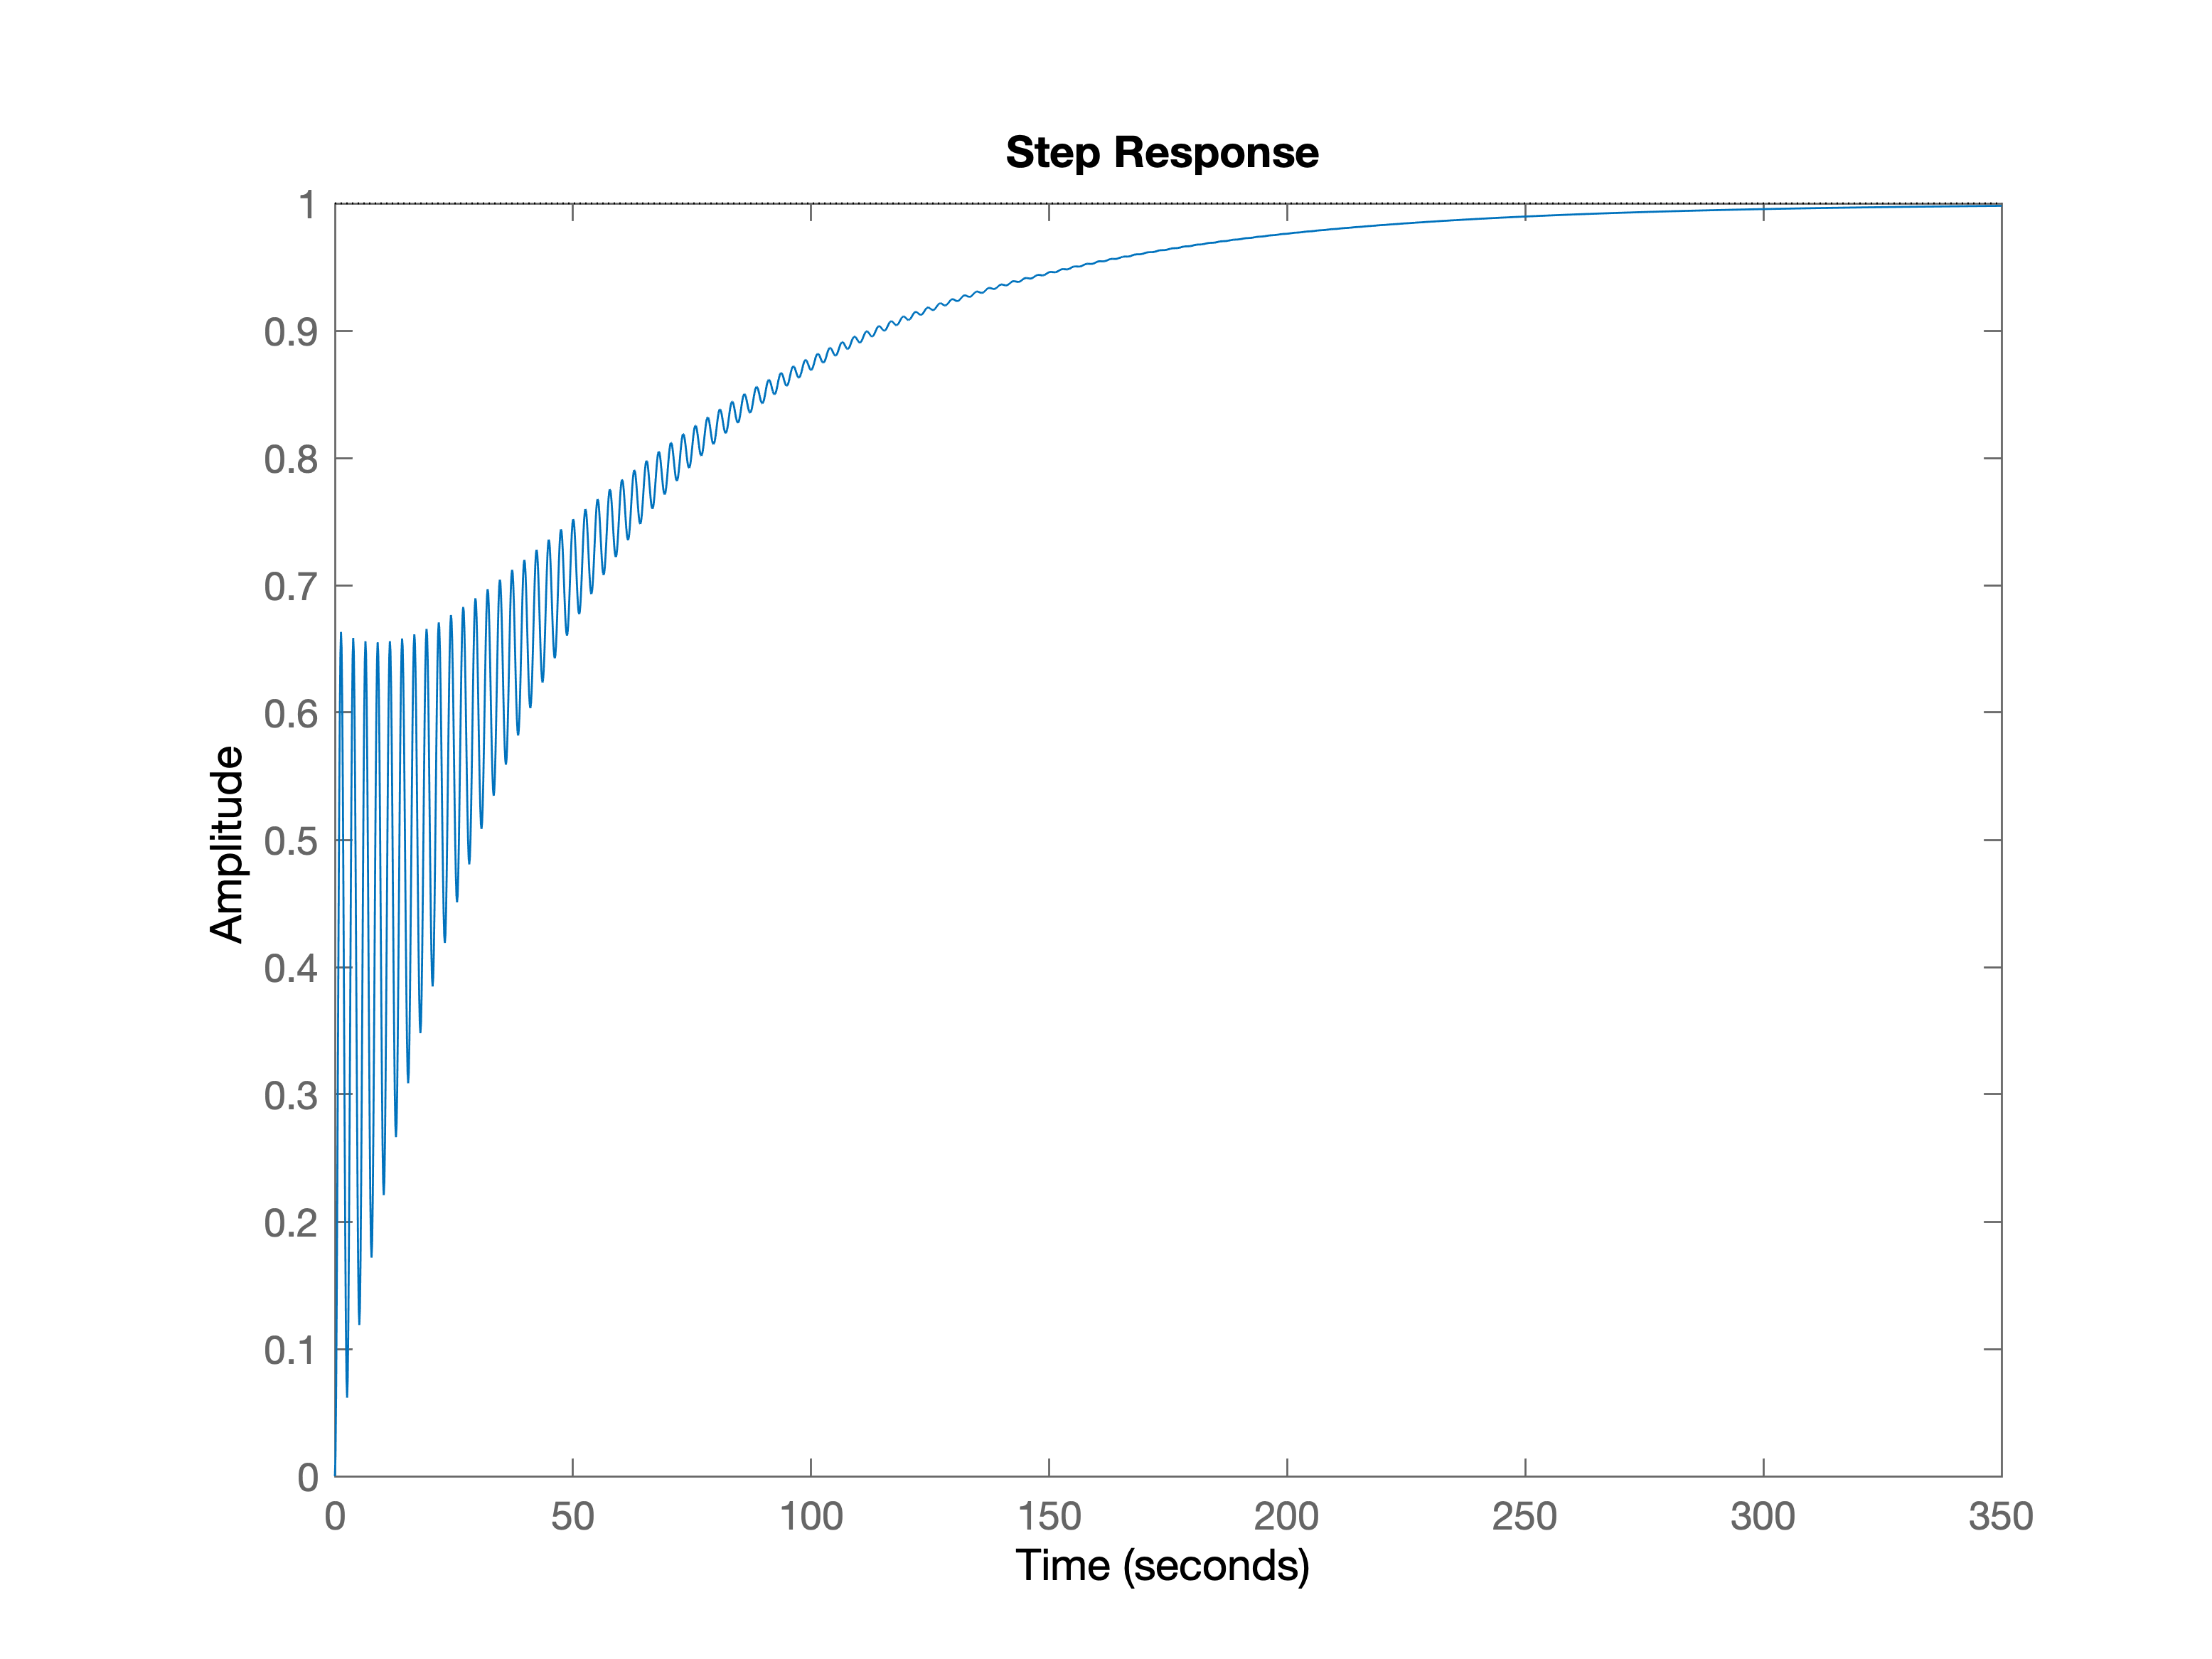
\includegraphics[width=12cm]{../Figure/Q1/Q1_system_respond.png}
    \end{figure}
    \item system root locus
    \begin{figure}[H]
        \caption{system root locus plot}
        \centering
        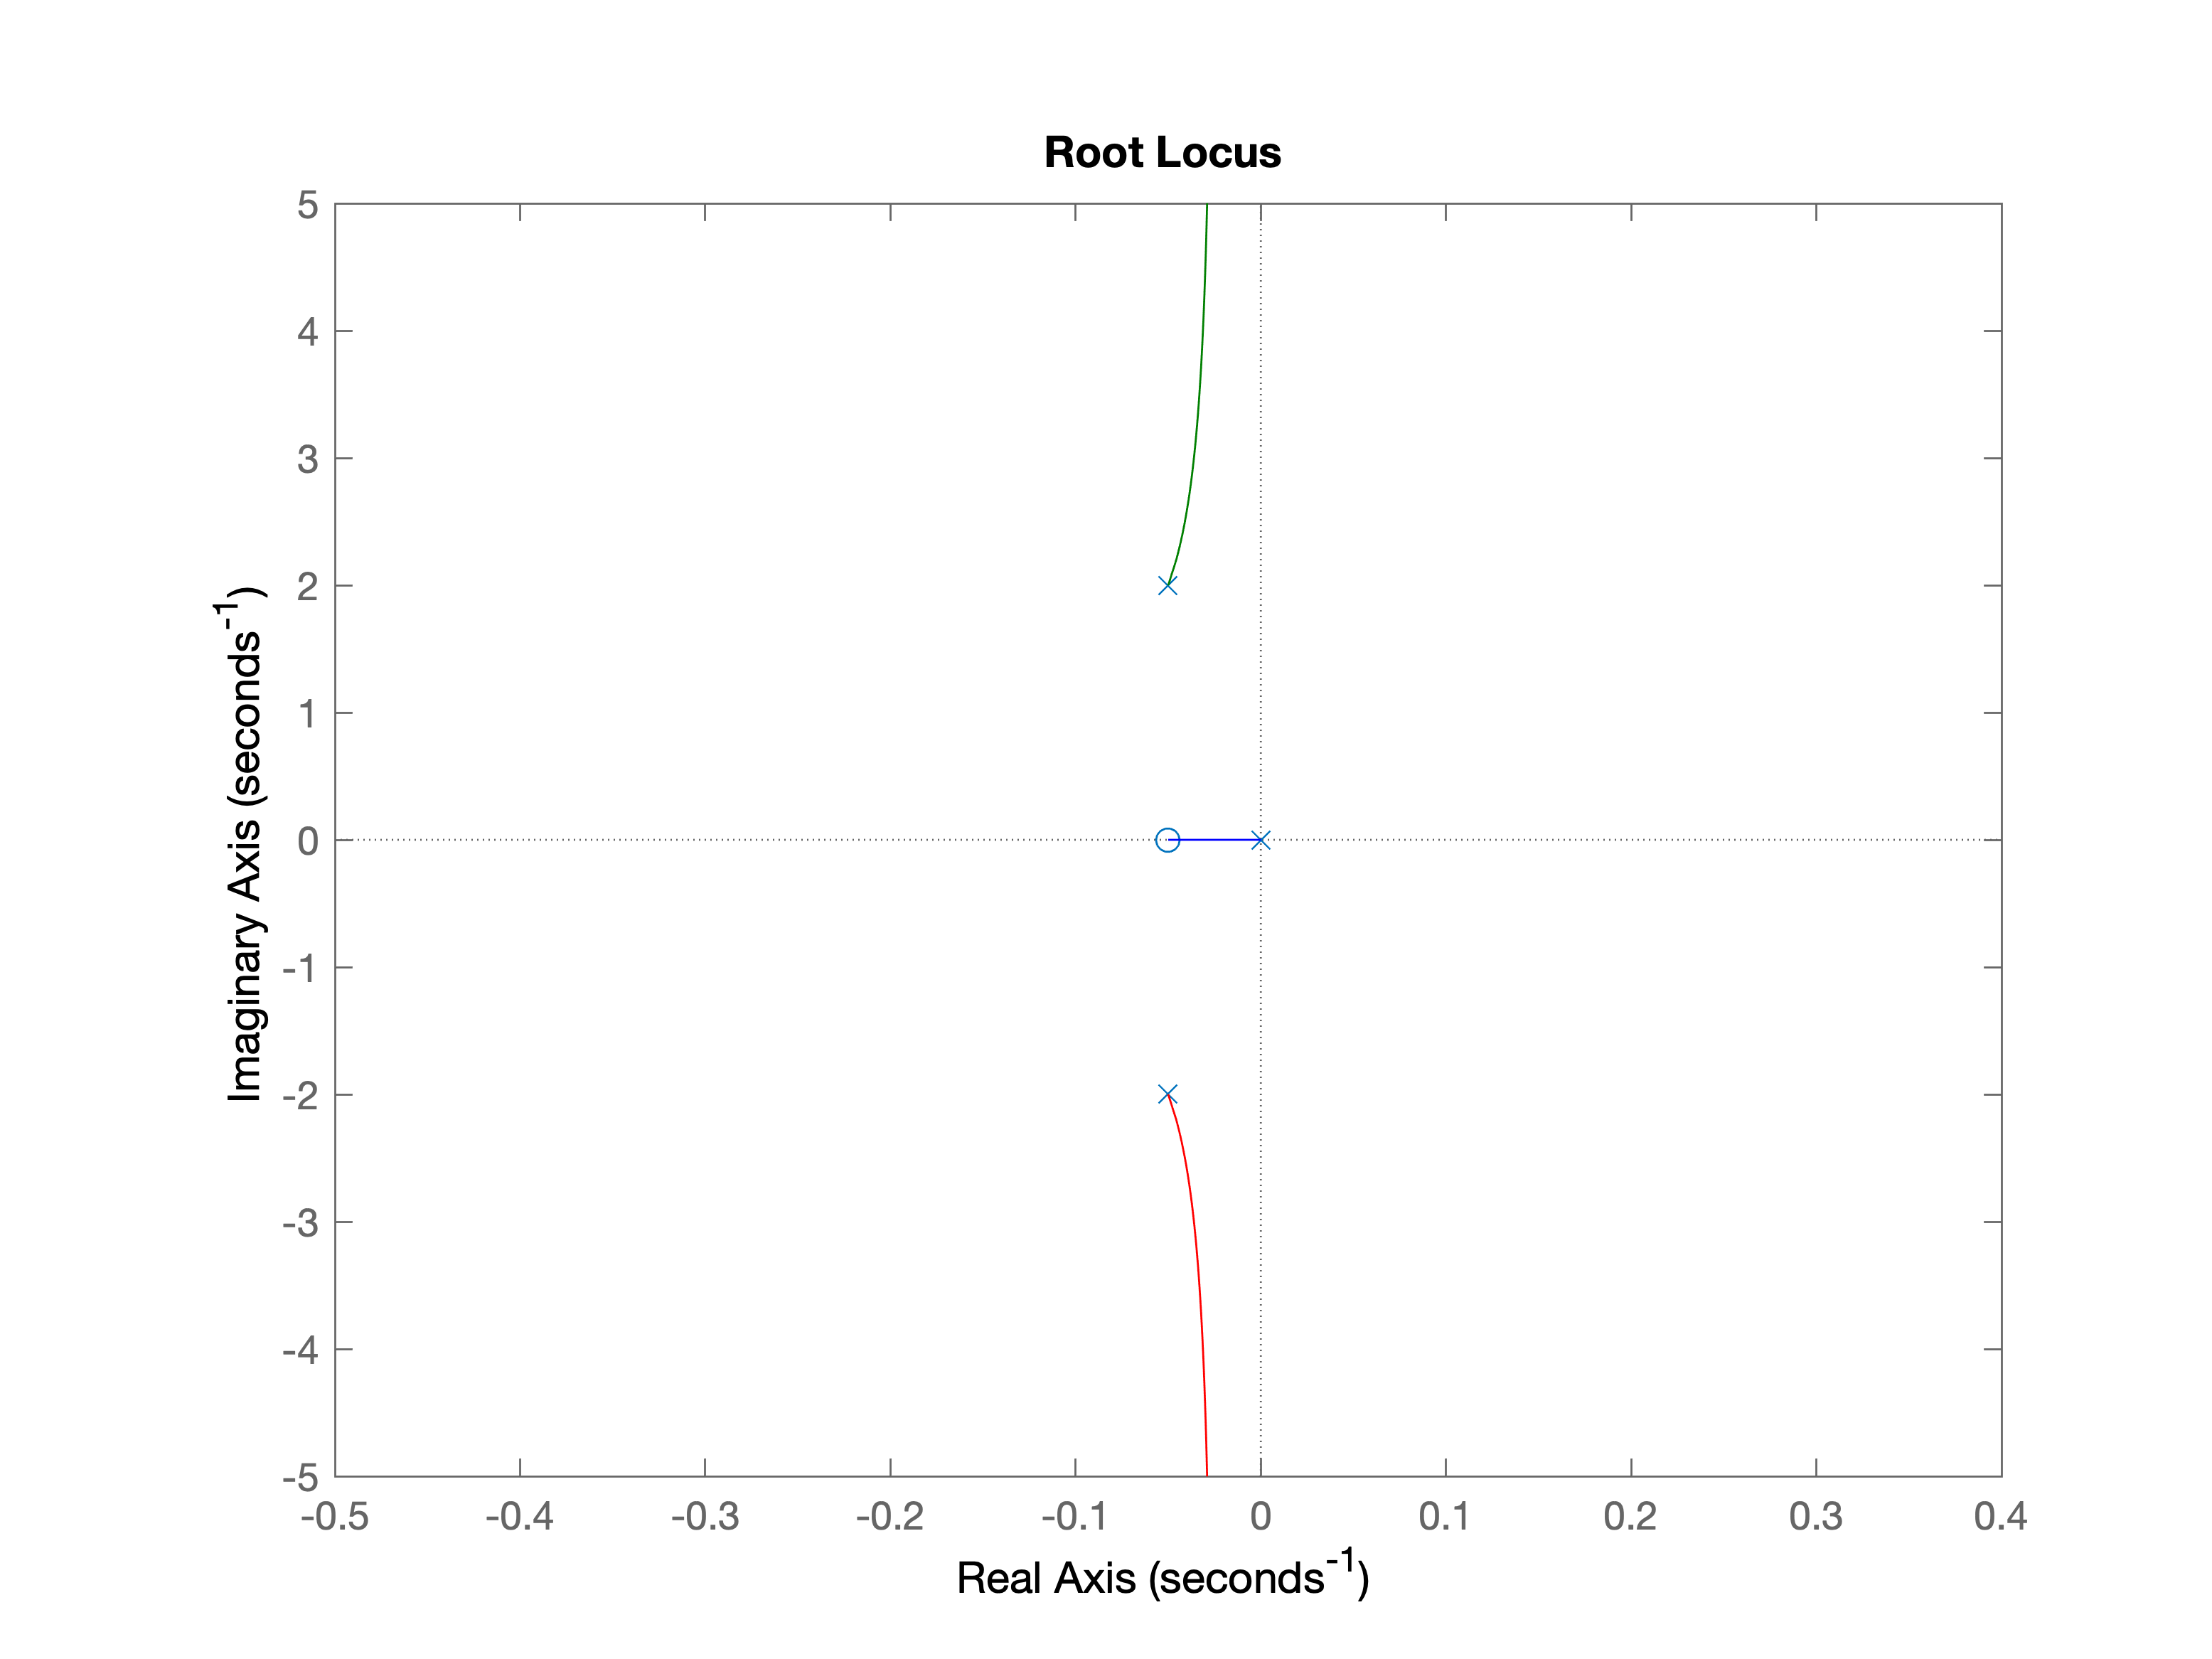
\includegraphics[width=12cm]{../Figure/Q1/Q1_system_rlocus.png}
    \end{figure}
    \item system with controller step responde
    \begin{figure}[H]
        \caption{system with controller step responde}
        \centering
        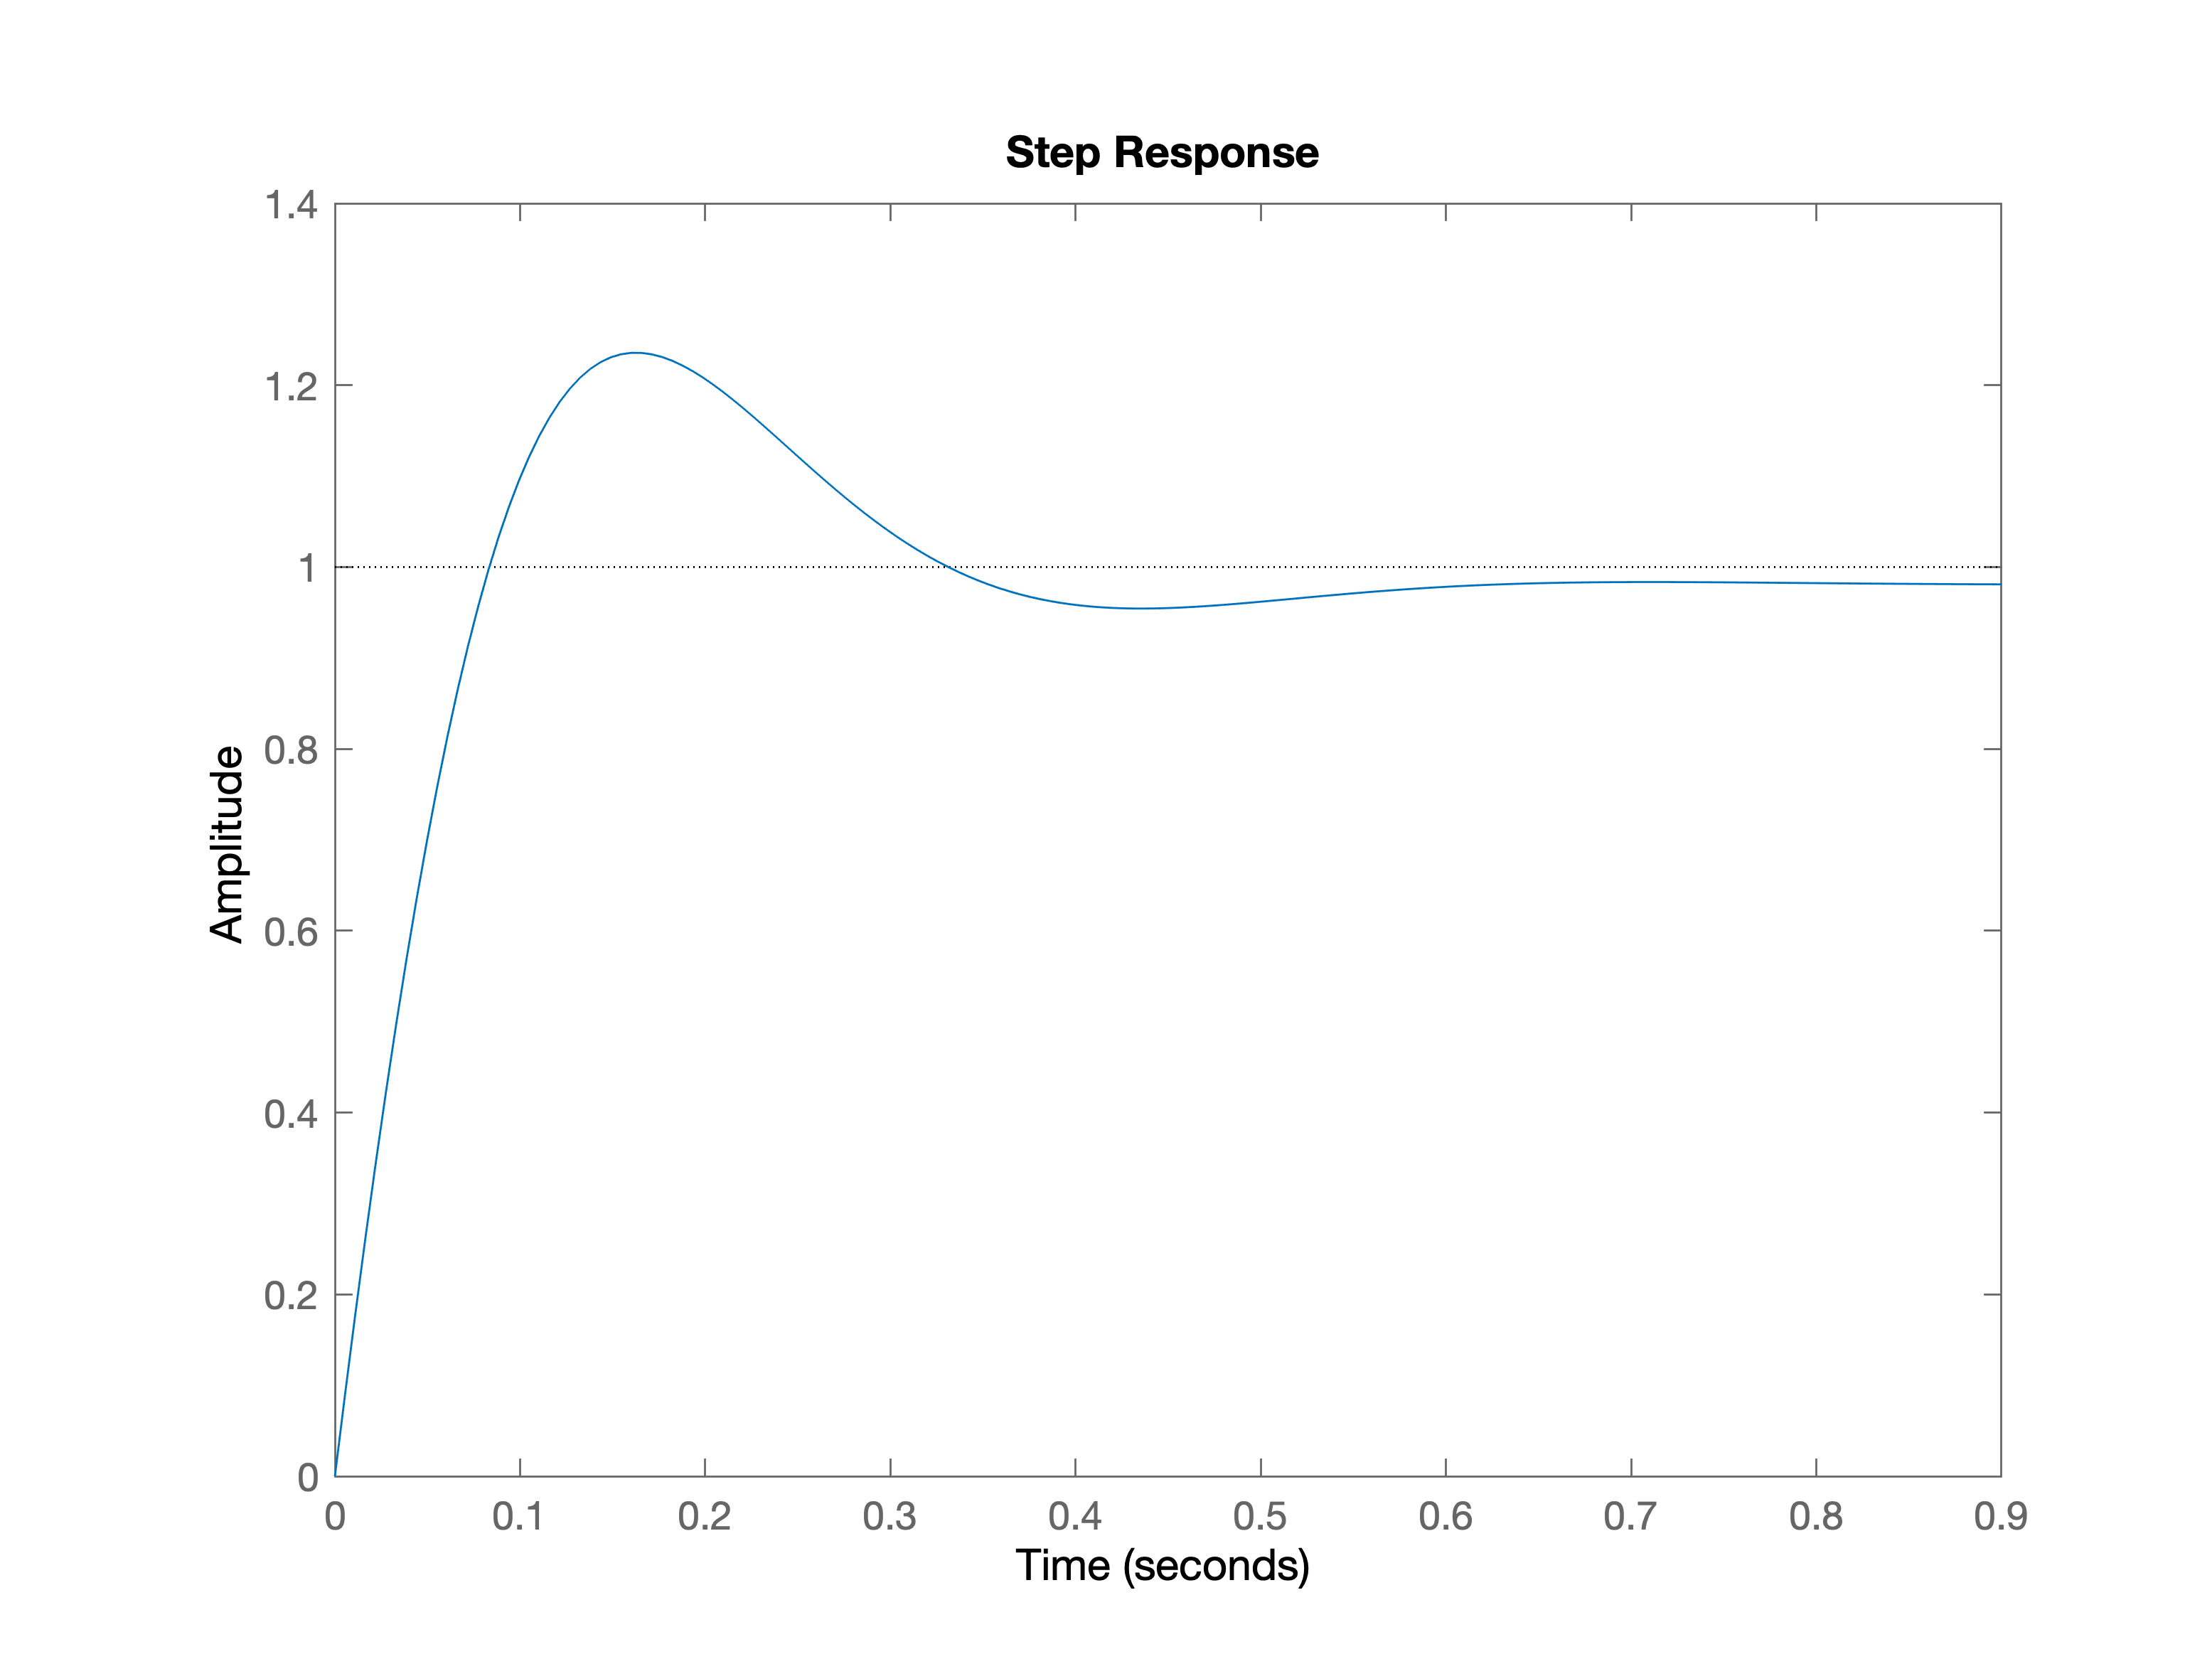
\includegraphics[width=12cm]{../Figure/Q1/Q1_system_controller_respond.png}
    \end{figure}
    \item system with controller root locus
    \begin{figure}[H]
        \caption{system with controller root locus plot}
        \centering
        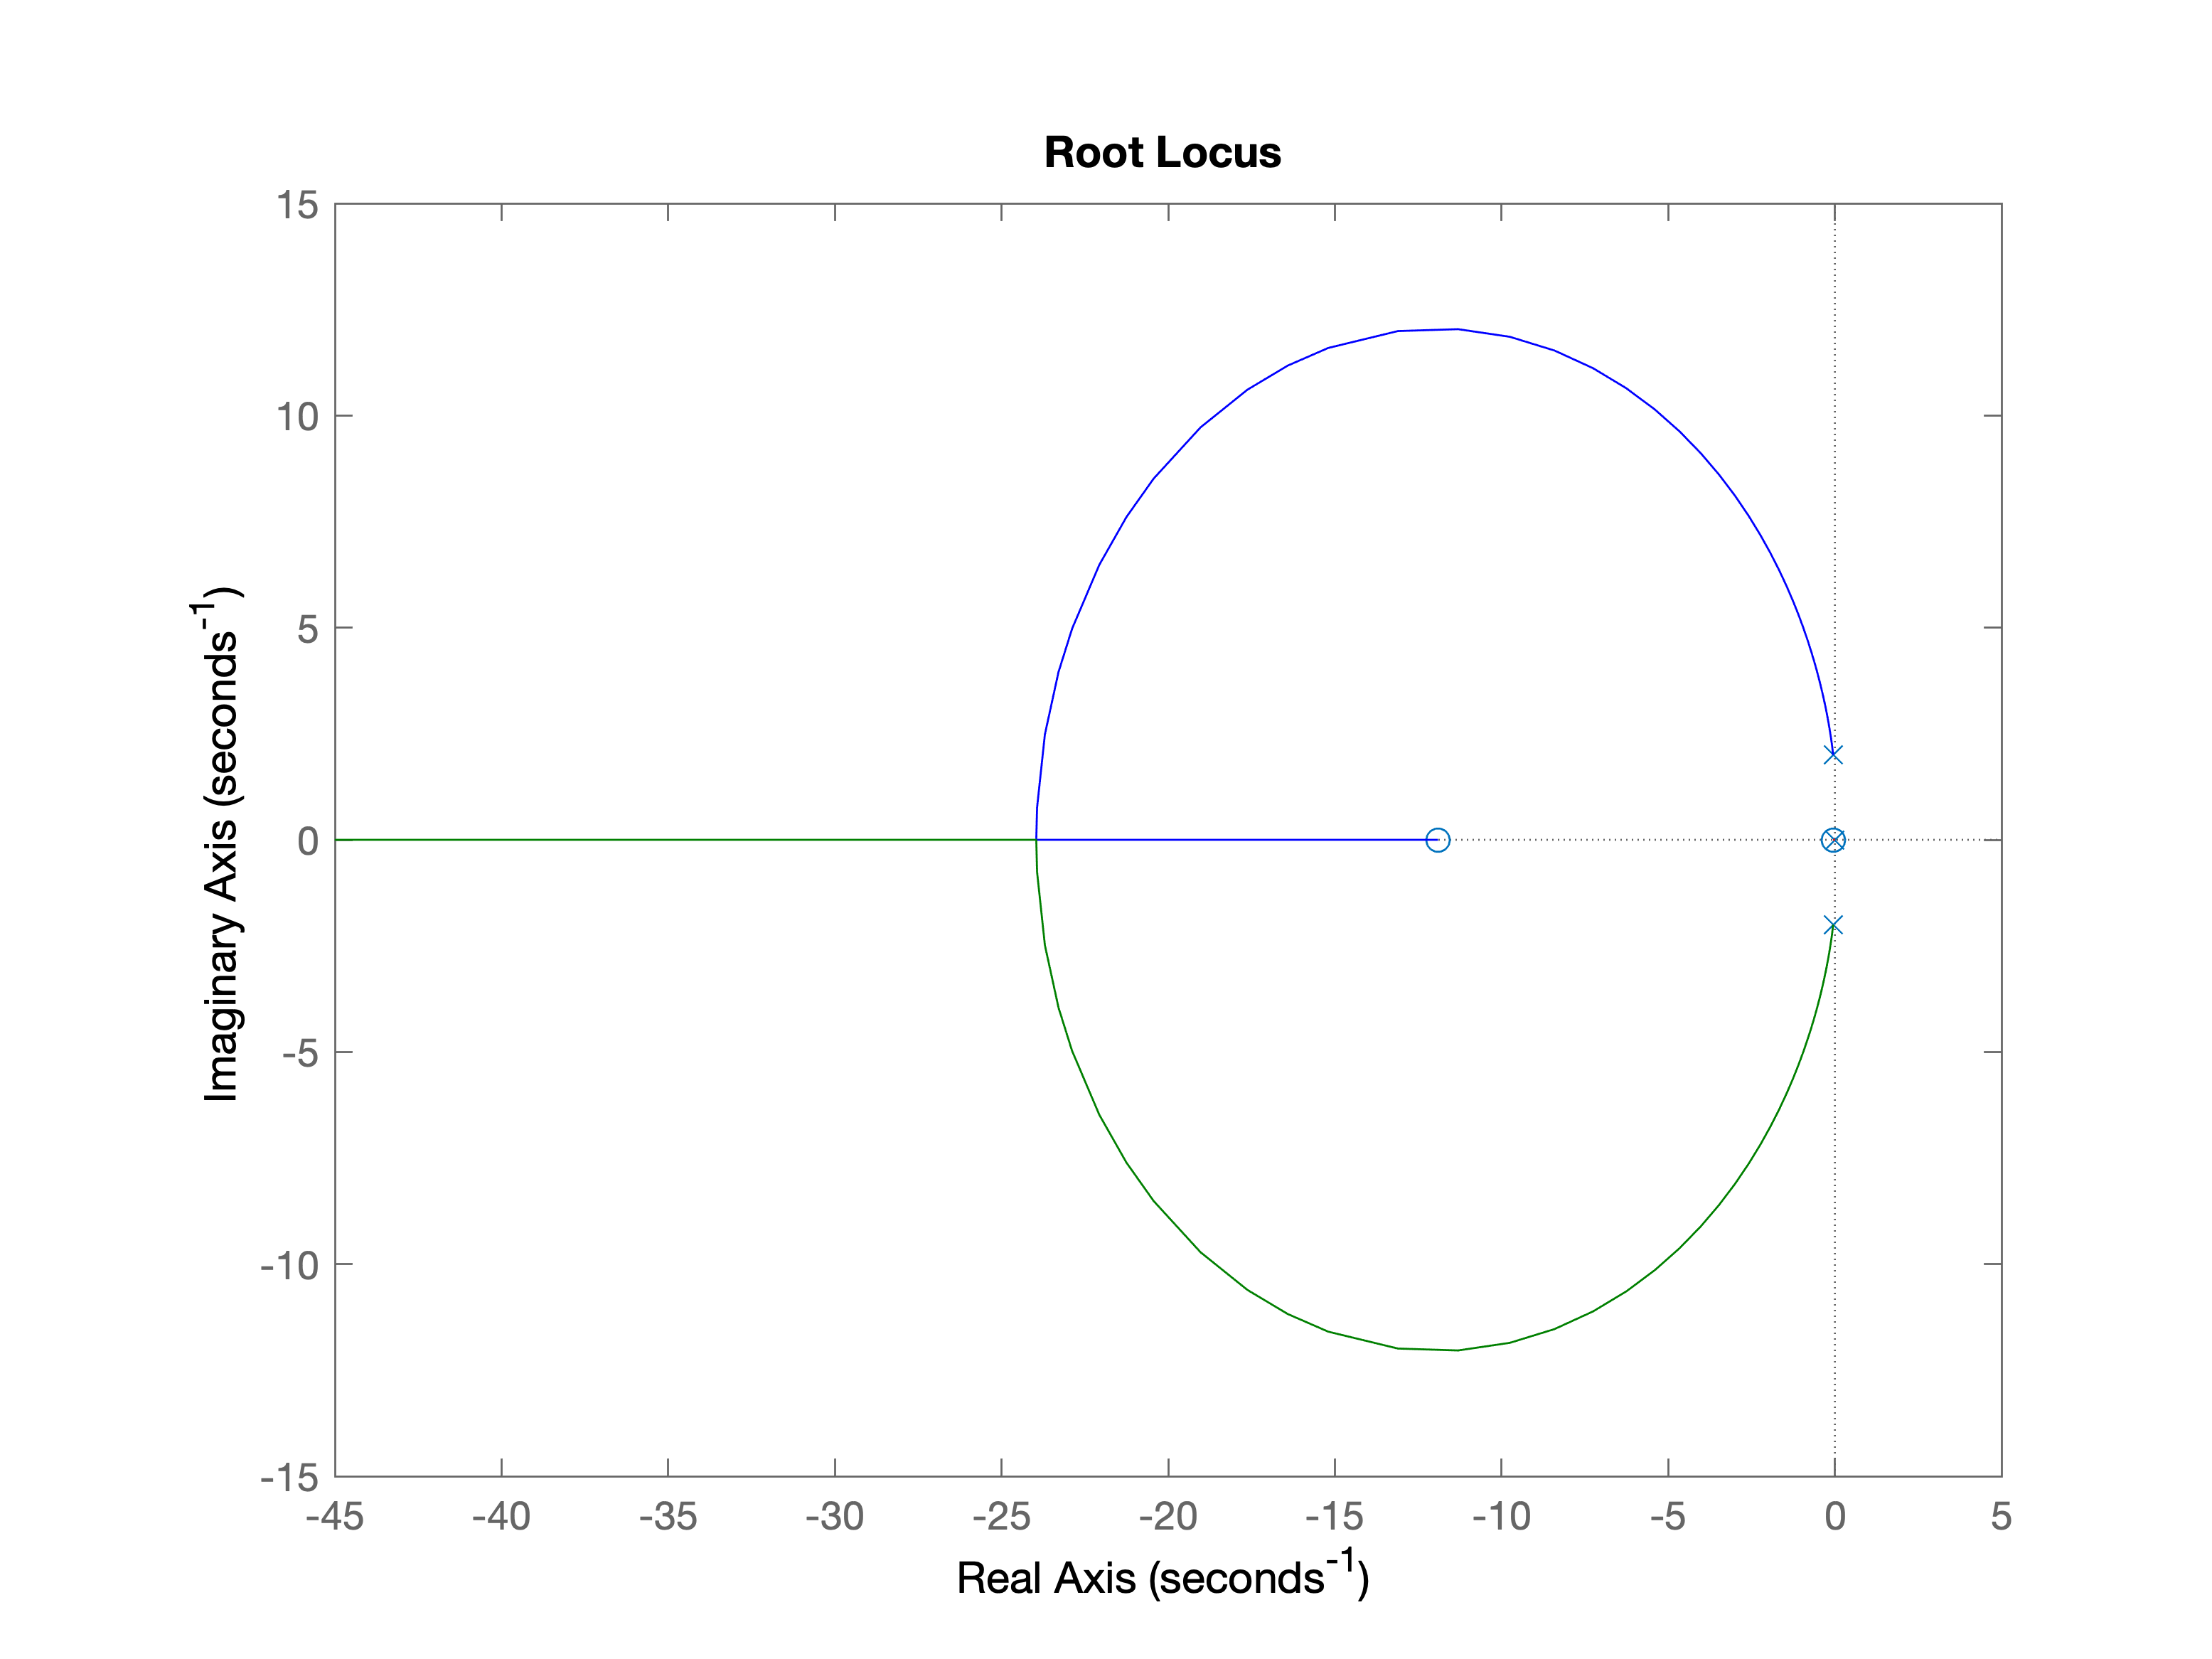
\includegraphics[width=12cm]{../Figure/Q1/Q1_system_controller_rlocus.png}
    \end{figure}
    \item system with and without controller step responde
    \begin{figure}[H]
        \caption{system with and without controller step responde}
        \centering
        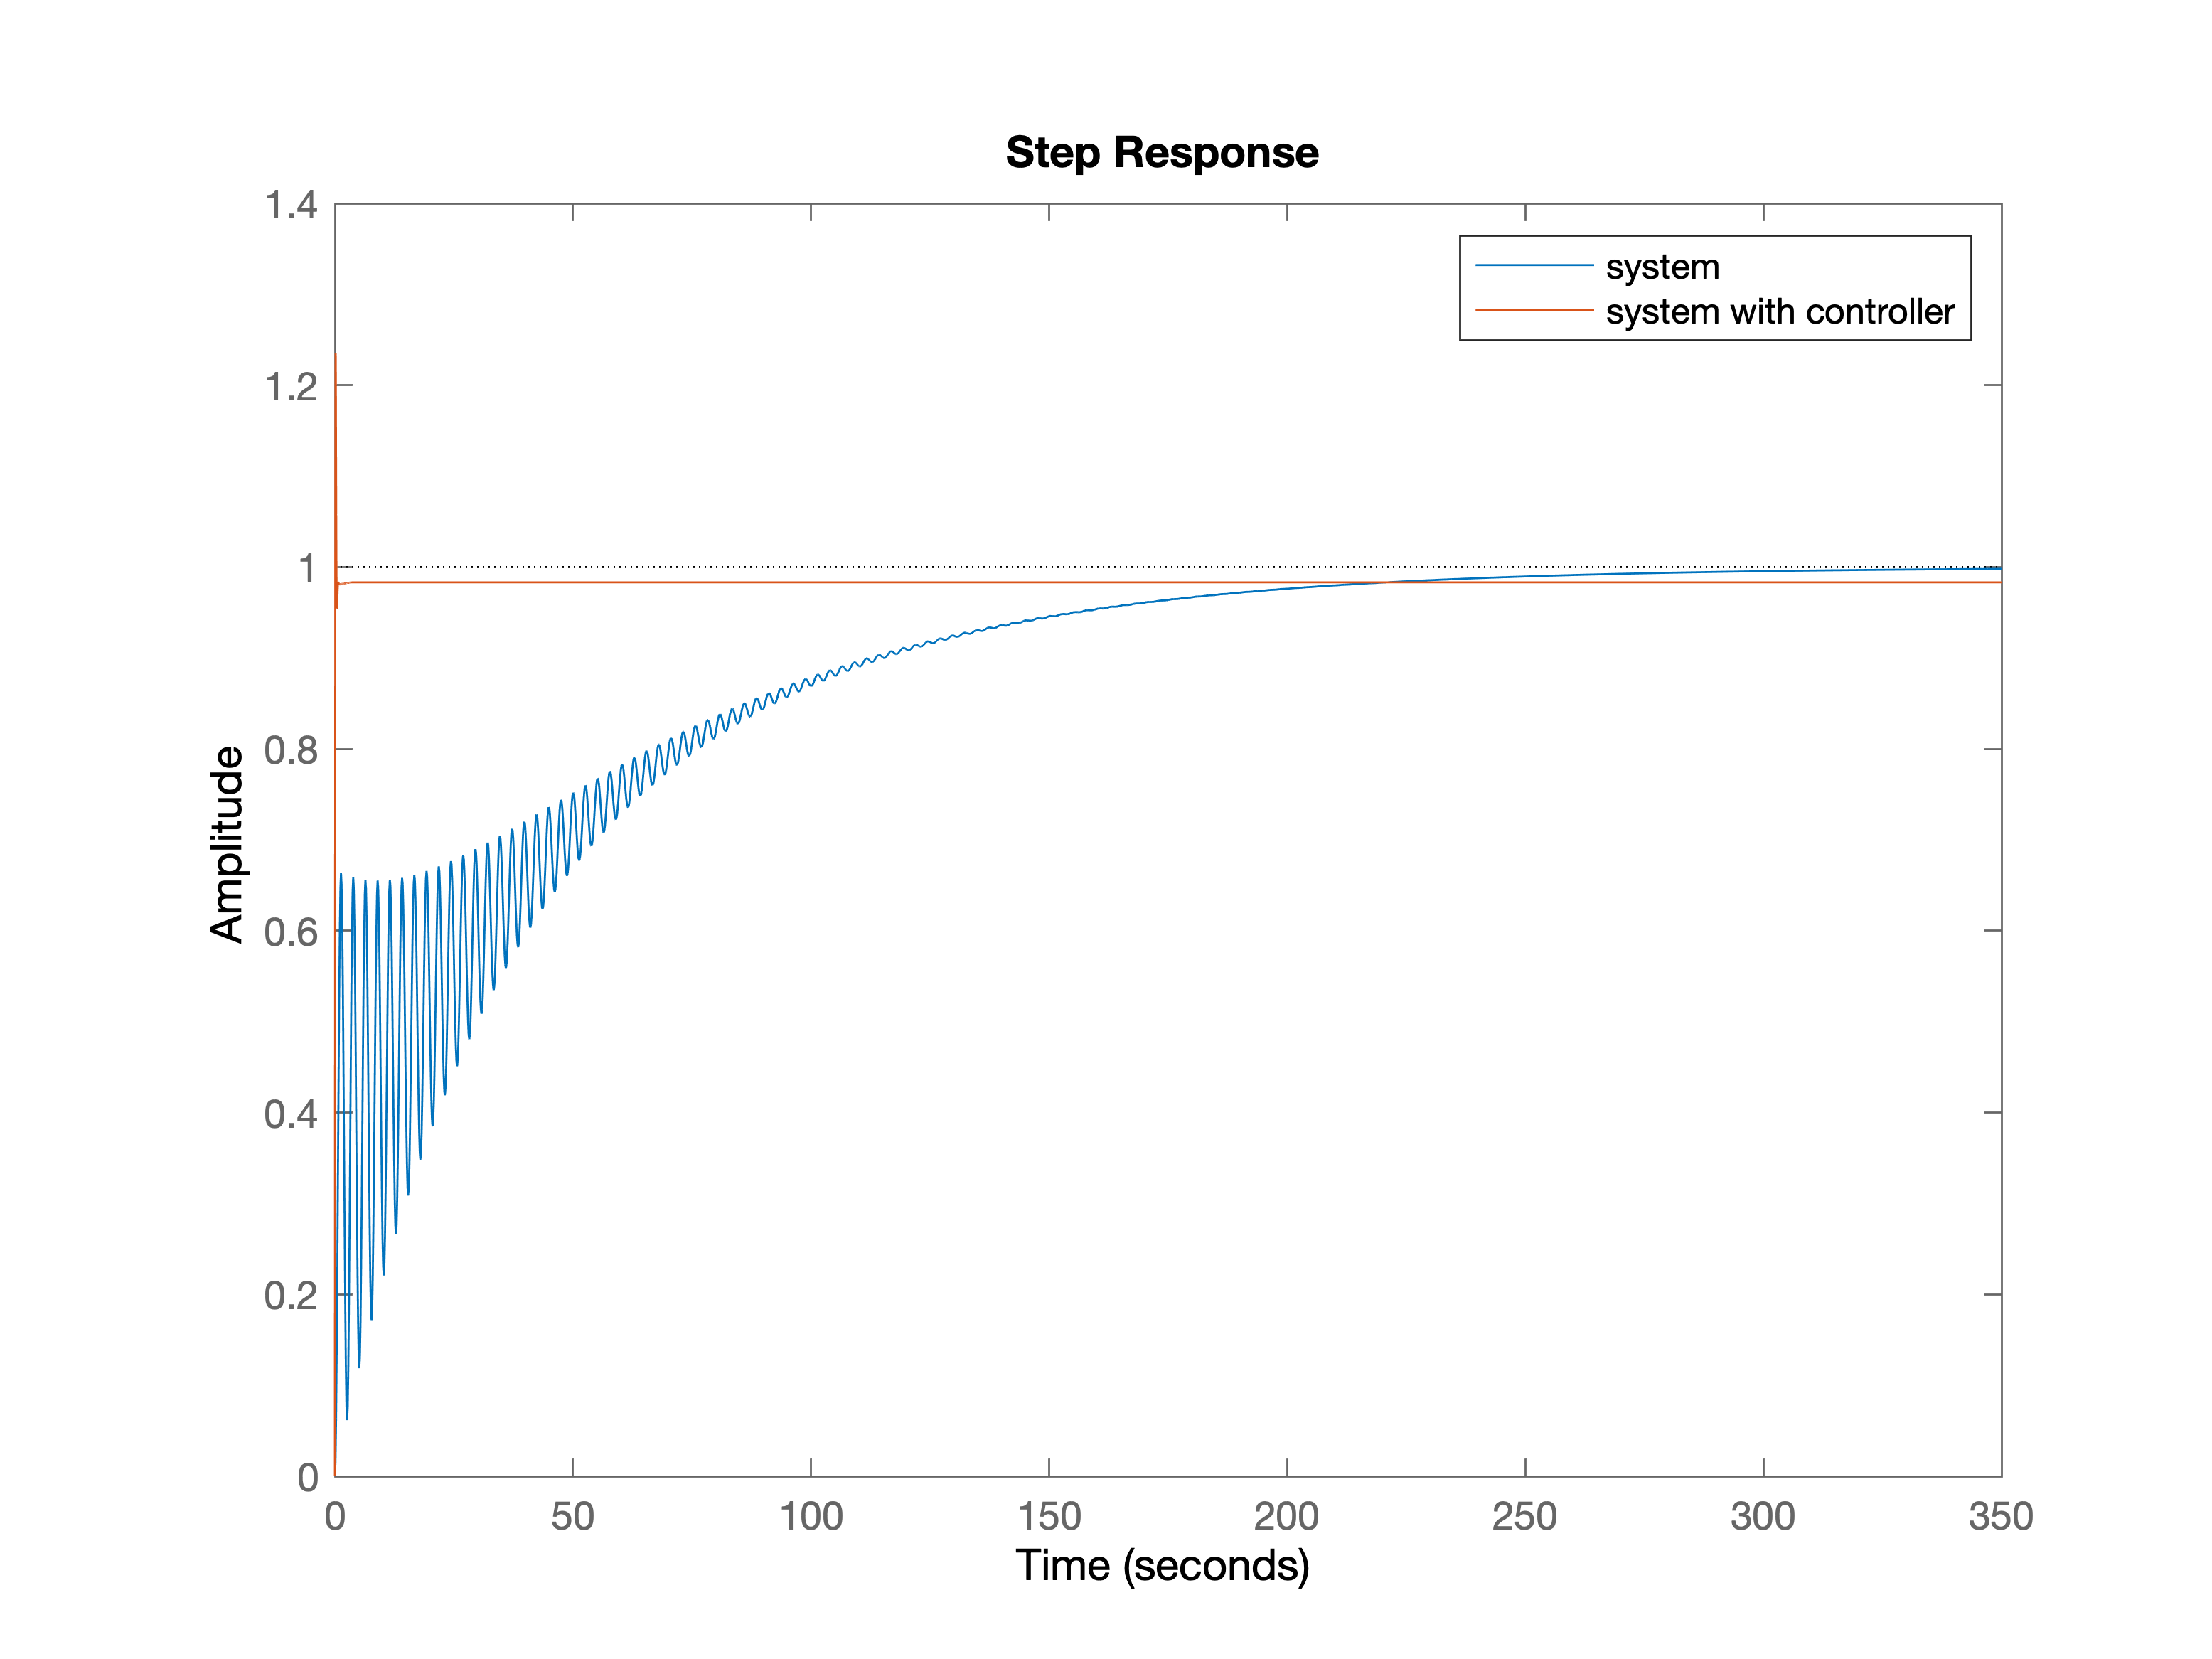
\includegraphics[width=12cm]{../Figure/Q1/Q1_respond_all.png}
    \end{figure}
    \item system with and without controller root locus
    \begin{figure}[H]
        \caption{system with and withou controller root locus plot}
        \centering
        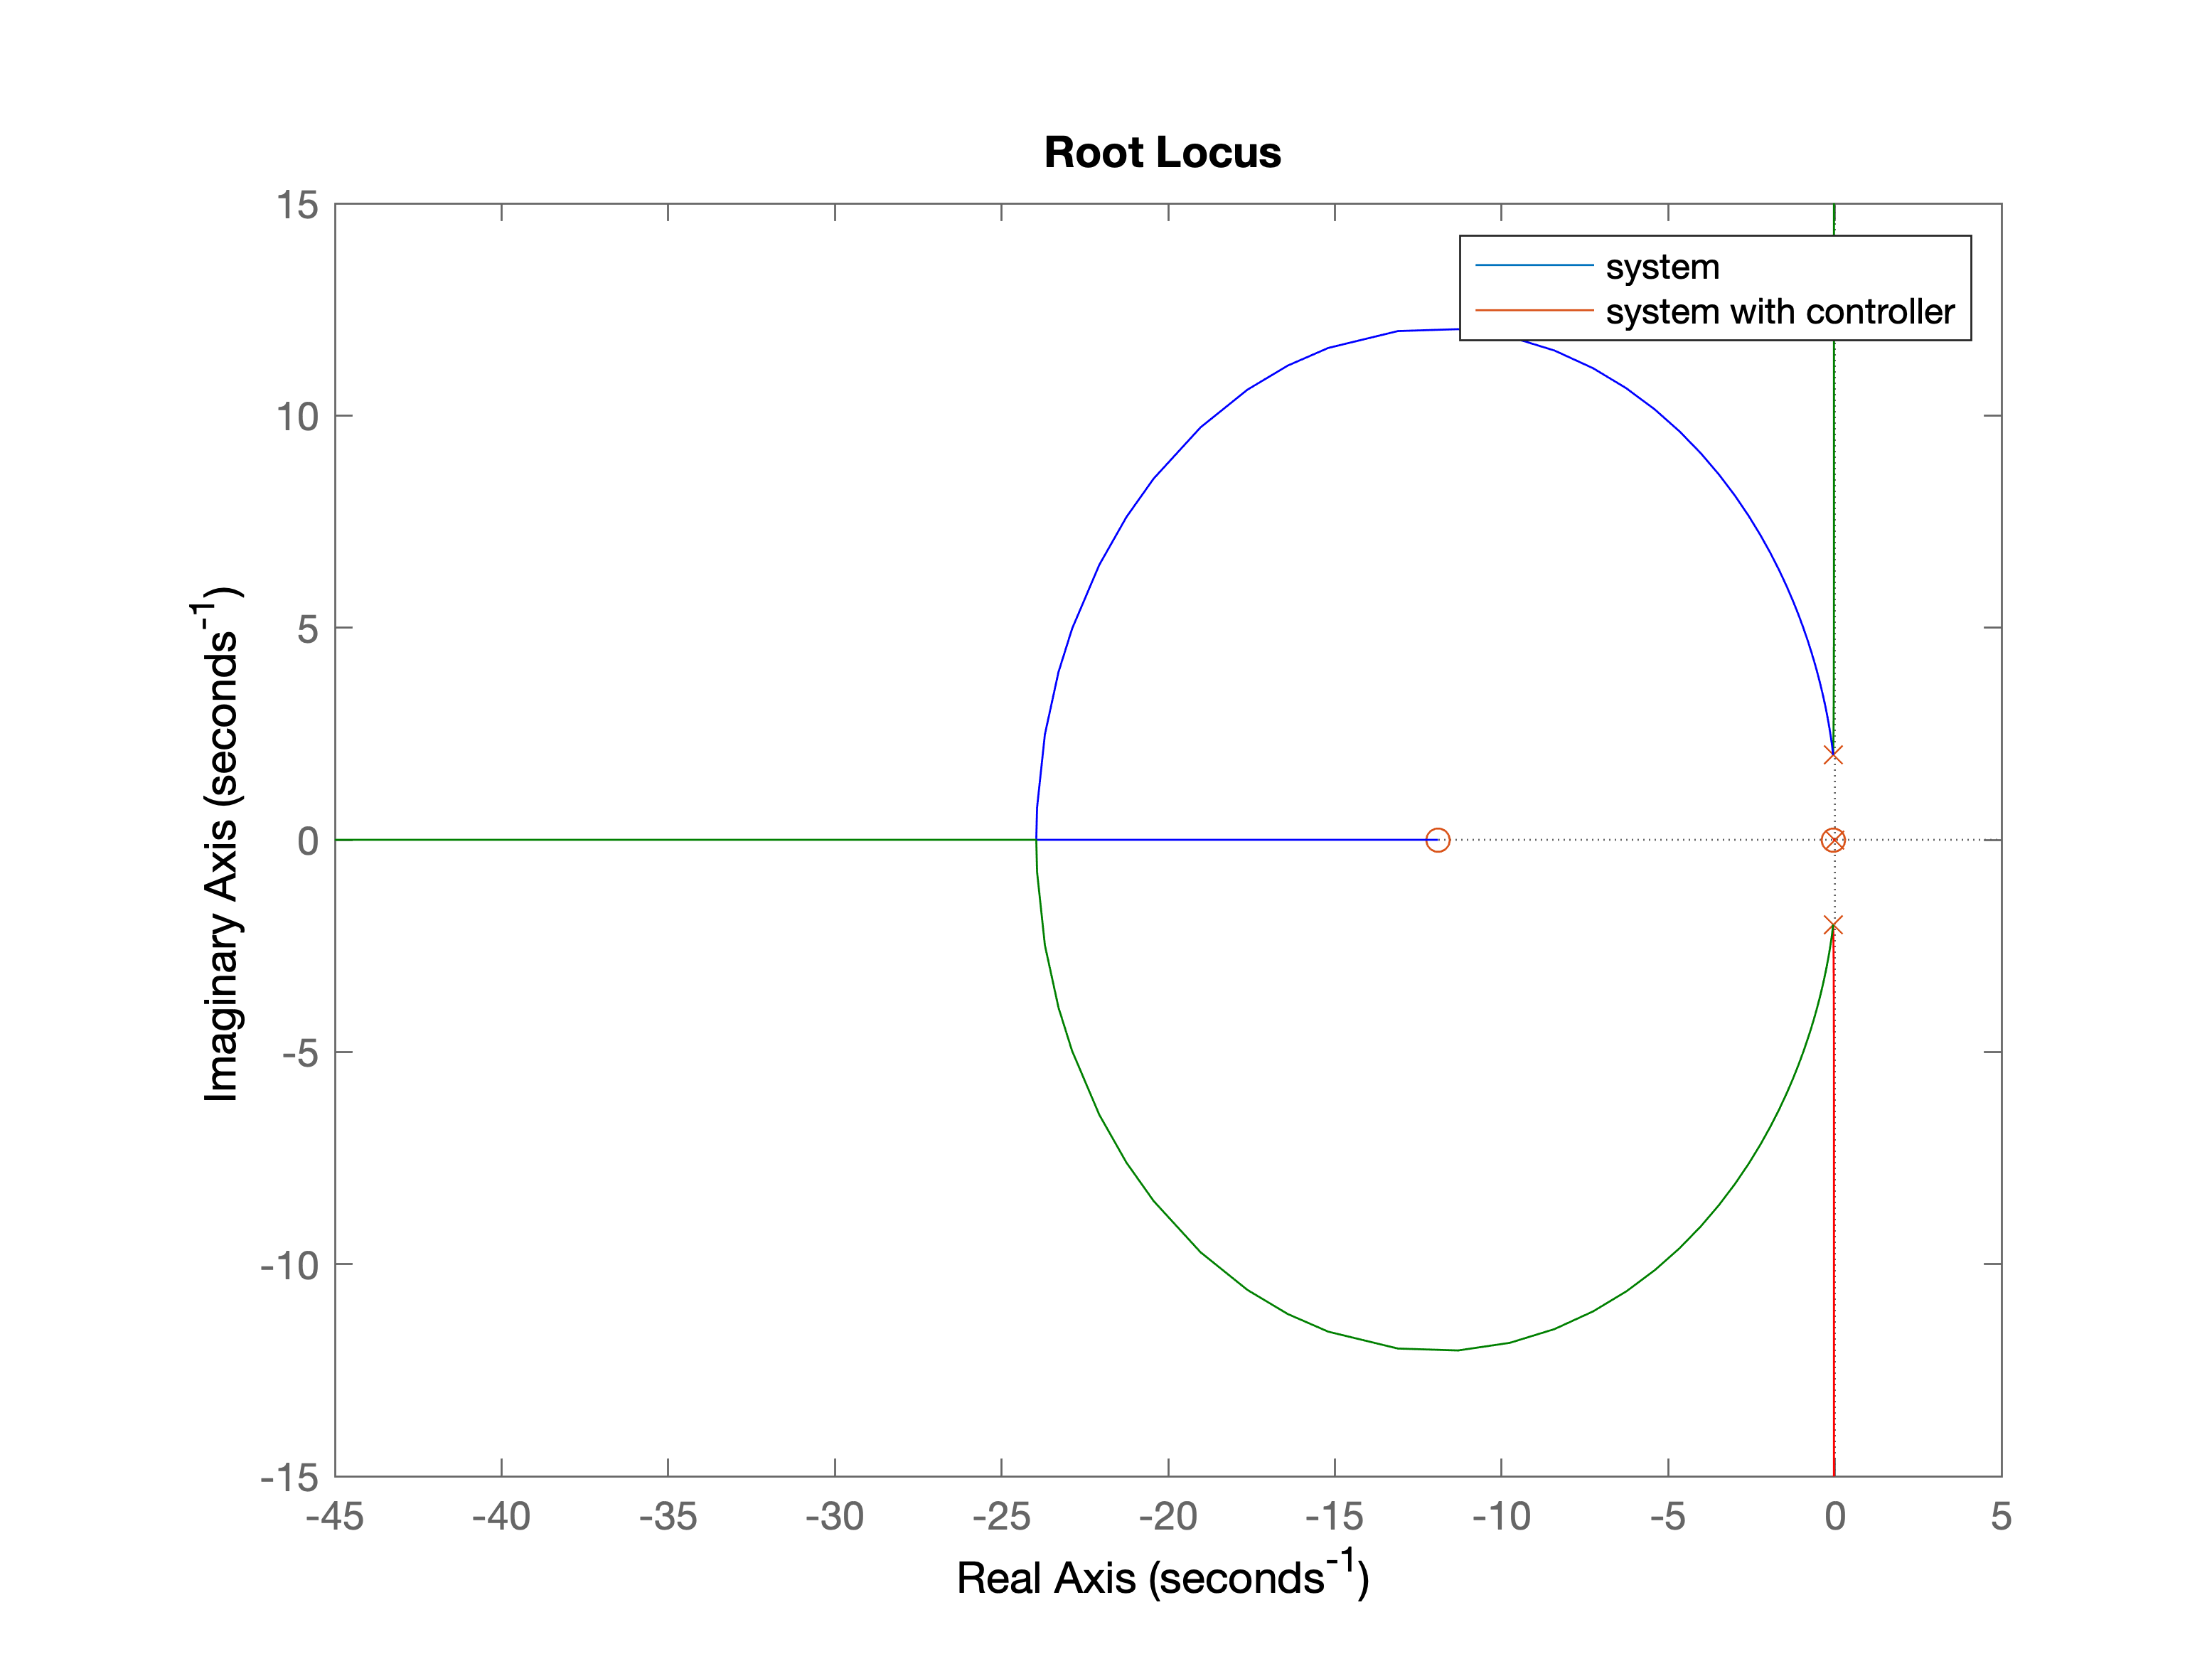
\includegraphics[width=12cm]{../Figure/Q1/Q1_rlocus.png}
    \end{figure}
\end{itemize}